\begin{figure}[h]
	\centering
	\captionsetup[subfigure]{labelformat=empty}
	%c1
	\begin{subfigure}[t]{.1\textwidth}
		\centering
		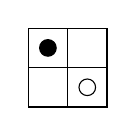
\begin{tikzpicture}[x=1cm]
			\draw (0,0)--(1,0)--(1,1)--(0,1)--cycle;
			\draw (.5,0)--(.5,.5)--(.5,1);
			\draw (0,.5)--(.5,.5)--(1,.5);
			\draw (.75,.25) circle (3pt);
			\filldraw (.25,.75) circle (3pt);
		\end{tikzpicture}
		\caption{$c_{1}$}
	\end{subfigure}%
	%c2
	\begin{subfigure}[t]{.1\textwidth}
		\centering
		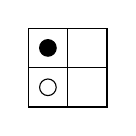
\begin{tikzpicture}[x=1cm]
			\draw (0,0)--(1,0)--(1,1)--(0,1)--cycle;
			\draw (.5,0)--(.5,.5)--(.5,1);
			\draw (0,.5)--(.5,.5)--(1,.5);
			\draw (.25,.25) circle (3pt);
			\filldraw (.25,.75) circle (3pt);
		\end{tikzpicture}
		\caption{$c_{2}$}
	\end{subfigure}%
	%c3
	\begin{subfigure}[t]{.1\textwidth}
		\centering
		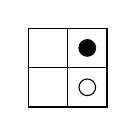
\begin{tikzpicture}[x=1cm]
			\draw (0,0)--(1,0)--(1,1)--(0,1)--cycle;
			\draw (.5,0)--(.5,.5)--(.5,1);
			\draw (0,.5)--(.5,.5)--(1,.5);
			\draw (.75,.25) circle (3pt);
			\filldraw (.75,.75) circle (3pt);
		\end{tikzpicture}
		\caption{$c_{3}$}
	\end{subfigure}%
	%c4
	\begin{subfigure}[t]{.1\textwidth}
		\centering
		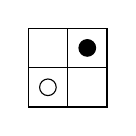
\begin{tikzpicture}[x=1cm]
			\draw (0,0)--(1,0)--(1,1)--(0,1)--cycle;
			\draw (.5,0)--(.5,.5)--(.5,1);
			\draw (0,.5)--(.5,.5)--(1,.5);
			\draw (.25,.25) circle (3pt);
			\filldraw (.75,.75) circle (3pt);
		\end{tikzpicture}
		\caption{$c_{4}$}
	\end{subfigure}%
	%c5
	\begin{subfigure}[t]{.1\textwidth}
		\centering
		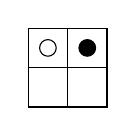
\begin{tikzpicture}[x=1cm]
			\draw (0,0)--(1,0)--(1,1)--(0,1)--cycle;
			\draw (.5,0)--(.5,.5)--(.5,1);
			\draw (0,.5)--(.5,.5)--(1,.5);
			\draw (.25,.75) circle (3pt);
			\filldraw (.75,.75) circle (3pt);
		\end{tikzpicture}
		\caption{$c_{5}$}
	\end{subfigure}%
	%c6
	\begin{subfigure}[t]{.1\textwidth}
		\centering
		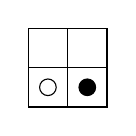
\begin{tikzpicture}[x=1cm]
			\draw (0,0)--(1,0)--(1,1)--(0,1)--cycle;
			\draw (.5,0)--(.5,.5)--(.5,1);
			\draw (0,.5)--(.5,.5)--(1,.5);
			\draw (.25,.25) circle (3pt);
			\filldraw (.75,.25) circle (3pt);
		\end{tikzpicture}
		\caption{$c_{6}$}
	\end{subfigure}
	
	%c7
	\begin{subfigure}[t]{.1\textwidth}
		\centering
		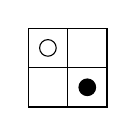
\begin{tikzpicture}[x=1cm]
			\draw (0,0)--(1,0)--(1,1)--(0,1)--cycle;
			\draw (.5,0)--(.5,.5)--(.5,1);
			\draw (0,.5)--(.5,.5)--(1,.5);
			\draw (.25,.75) circle (3pt);
			\filldraw (.75,.25) circle (3pt);
		\end{tikzpicture}
		\caption{$c_{7}$}
	\end{subfigure}%
	%c8
	\begin{subfigure}[t]{.1\textwidth}
		\centering
		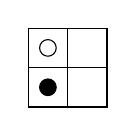
\begin{tikzpicture}[x=1cm]
			\draw (0,0)--(1,0)--(1,1)--(0,1)--cycle;
			\draw (.5,0)--(.5,.5)--(.5,1);
			\draw (0,.5)--(.5,.5)--(1,.5);
			\draw (.25,.75) circle (3pt);
			\filldraw (.25,.25) circle (3pt);
		\end{tikzpicture}
		\caption{$c_{8}$}
	\end{subfigure}%
	%c9
	\begin{subfigure}[t]{.1\textwidth}
		\centering
		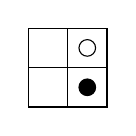
\begin{tikzpicture}[x=1cm]
			\draw (0,0)--(1,0)--(1,1)--(0,1)--cycle;
			\draw (.5,0)--(.5,.5)--(.5,1);
			\draw (0,.5)--(.5,.5)--(1,.5);
			\draw (.75,.75) circle (3pt);
			\filldraw (.75,.25) circle (3pt);
		\end{tikzpicture}
		\caption{$c_{9}$}
	\end{subfigure}%
	%c10
	\begin{subfigure}[t]{.1\textwidth}
		\centering
		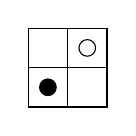
\begin{tikzpicture}[x=1cm]
			\draw (0,0)--(1,0)--(1,1)--(0,1)--cycle;
			\draw (.5,0)--(.5,.5)--(.5,1);
			\draw (0,.5)--(.5,.5)--(1,.5);
			\draw (.75,.75) circle (3pt);
			\filldraw (.25,.25) circle (3pt);
		\end{tikzpicture}
		\caption{$c_{10}$}
	\end{subfigure}%
	%c11
	\begin{subfigure}[t]{.1\textwidth}
		\centering
		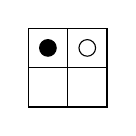
\begin{tikzpicture}[x=1cm]
			\draw (0,0)--(1,0)--(1,1)--(0,1)--cycle;
			\draw (.5,0)--(.5,.5)--(.5,1);
			\draw (0,.5)--(.5,.5)--(1,.5);
			\draw (.75,.75) circle (3pt);
			\filldraw (.25,.75) circle (3pt);
		\end{tikzpicture}
		\caption{$c_{11}$}
	\end{subfigure}%
	%c12
	\begin{subfigure}[t]{.1\textwidth}
		\centering
		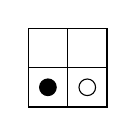
\begin{tikzpicture}[x=1cm]
			\draw (0,0)--(1,0)--(1,1)--(0,1)--cycle;
			\draw (.5,0)--(.5,.5)--(.5,1);
			\draw (0,.5)--(.5,.5)--(1,.5);
			\draw (.75,.25) circle (3pt);
			\filldraw (.25,.25) circle (3pt);
		\end{tikzpicture}
		\caption{$c_{12}$}
	\end{subfigure}
	
	%D
	\begin{subfigure}[b]{\textwidth}
		\centering
		\[D:
		\raisebox{-.5\height}
		{
			\begin{tikzpicture}[every edge/.style={draw,postaction={decorate,decoration={markings,mark=at position 0.5 with {\arrow[scale=2]{>}}}}}]
				\foreach \i/\j in {0/12,1/11,2/10,3/9,4/8,5/7,6/6,7/5,8/4,-3/3,-2/2,-1/1} {
					\setcounter{Angle}{90 + \i * 360 / 12};
					\vertex (c\j) at (\theAngle:2) [label=\theAngle:$c_{\j}$]{};
				}
				\path
					(c1) edge[bend right=40] (c3)
					(c1) edge[bend left=40] (c11)
					(c2) edge (c1)
					(c2) edge[bend right=40] (c4)
					(c4) edge (c3)
					(c4) edge (c5)
					(c6) edge[bend left=40] (c4)
					(c6) edge (c7)
					(c7) edge[bend left=40] (c5)
					(c7) edge[bend right=40] (c9)
					(c8) edge (c7)
					(c8) edge[bend right=40] (c10)
					(c10) edge (c9)
					(c10) edge (c11)
					(c12) edge[bend left=40] (c10)
					(c12) edge (c1)
				;
			\end{tikzpicture}
		}\]
	\end{subfigure}
	\caption{Modeling twelve configurations by a digraph}
\end{figure}